% -*- mode: latex; mode: flyspell; ispell-local-dictionary: "en_US"; coding: utf-8; fill-column: 80 -*-

\documentclass{article}

\usepackage[utf8]{inputenc}
\usepackage[english]{babel}

\usepackage{amsmath,amsfonts,amssymb}
\usepackage{fullpage}
\usepackage{verbatim}

\usepackage{tikz,pgfplots}
\usetikzlibrary{patterns, patterns.meta}
\usepgfplotslibrary{groupplots}

\makeatletter
\newcommand{\resetplotspccsmallhuff}{
  \makeatletter
  \pgfplots@stacked@isfirstplottrue
  \makeatother
  \addplot[forget plot, draw = none] coordinates {(dna, 0) (pitches, 0) (sources, 0)};
}
\newcommand{\resetplotspcclargehuff}{
  \makeatletter
  \pgfplots@stacked@isfirstplottrue
  \makeatother
  \addplot[forget plot, draw = none] coordinates {(dblp.xml, 0) (english, 0) (proteins, 0)};
}
\makeatother


\pgfplotsset{
  /pgfplots/bar cycle list/.style = {
    /pgfplots/cycle list = {
      { fill = black!15, mark = none }
    }
  }
}

\pgfplotsset{
  major grid style = { thin, dotted, color = black!50 },
  minor grid style = { thin, dotted, color = black!50 },
  grid,
  xtick distance = 1,
  ymin = 0,
  every axis/.append style = {
    line width = 0.5pt,
    tick style = {
      line cap = round,
      thin,
      major tick length = 4pt,
      minor tick length = 2pt,
    },
  },
  legend cell align = left,
	/pgfplots/ybar legend/.style = {
		/pgfplots/legend image code/.code={%
			\draw[##1,/tikz/.cd,yshift=-0.25em]
			(0cm,0cm) rectangle (3pt,0.8em);},
	},  
}

\begin{document}

\title{WT Benchmark}
\author{Jan-Philipp Tarnowski}
\maketitle


% IMPORT-DATA stats  ../results-huff-pcc-2.out

% SQL UPDATE stats SET type = 'lwt-huff-pext-16-4', ds_order = 0 WHERE type LIKE 'lwt_huffman_pext_16_4'
% SQL UPDATE stats SET type = 'lwt-huff-shuffle-8-8', ds_order = 1 WHERE type LIKE 'lwt_huffman_shuffle_8_8'
% SQL UPDATE stats SET type = 'lwt-huff-shuffle-16-8', ds_order = 2 WHERE type LIKE 'lwt_huffman_shuffle_16_8'
% SQL UPDATE stats SET type = 'lwt-huff-shuffle-32-8', ds_order = 3 WHERE type LIKE 'lwt_huffman_shuffle_32_8'
% SQL UPDATE stats SET type = 'lwt-huff-shuffle-64-8', ds_order = 4 WHERE type LIKE 'lwt_huffman_shuffle_64_8'

% SQL UPDATE stats SET type = 'wm-huff-pext-16-4', ds_order = 8 WHERE type LIKE 'wm_huffman_pext_16_4'
% SQL UPDATE stats SET type = 'wm-huff-shuffle-8-8', ds_order = 9 WHERE type LIKE 'wm_huffman_shuffle_8_8'
% SQL UPDATE stats SET type = 'wm-huff-shuffle-16-8', ds_order = 10 WHERE type LIKE 'wm_huffman_shuffle_16_8'
% SQL UPDATE stats SET type = 'wm-huff-shuffle-32-8', ds_order = 11 WHERE type LIKE 'wm_huffman_shuffle_32_8'
% SQL UPDATE stats SET type = 'wm-huff-shuffle-64-8', ds_order = 12 WHERE type LIKE 'wm_huffman_shuffle_64_8'

% SQL DELETE FROM stats WHERE type LIKE '%\_%' ESCAPE '\'

% SQL UPDATE stats SET file = 'dblp.xml' WHERE file LIKE '%/dblp.xml'
% SQL UPDATE stats SET file = 'dna' WHERE file LIKE '%/dna'
% SQL UPDATE stats SET file = 'english' WHERE file LIKE '%/english'
% SQL UPDATE stats SET file = 'pitches' WHERE file LIKE '%/pitches'
% SQL UPDATE stats SET file = 'proteins' WHERE file LIKE '%/proteins'
% SQL UPDATE stats SET file = 'sources' WHERE file LIKE '%/sources'

\clearpage

\begin{center}
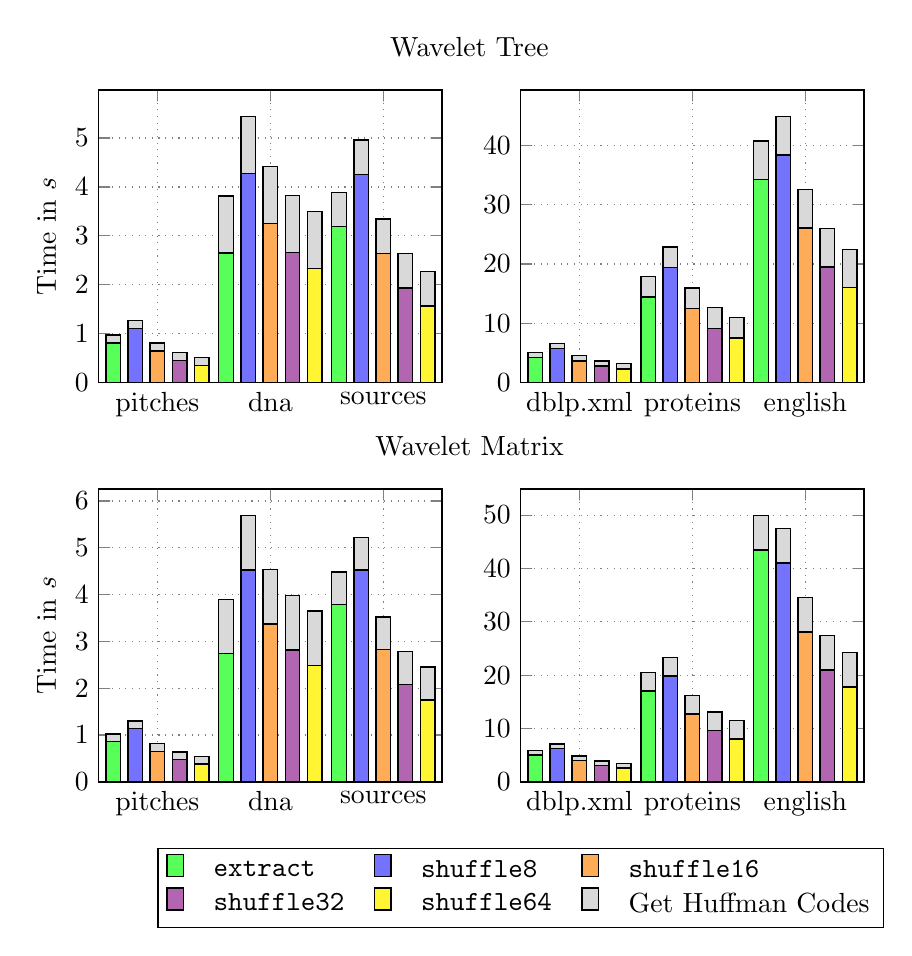
\begin{tikzpicture}
  \begin{groupplot} [
    width = 0.49\textwidth,
    height = 5.3cm,
    ybar stacked,
    enlarge x limits = 0.26,
    group style = { 
        vertical sep = 1.35cm,
        group size = { 
            2 by 2
        } 
    },
    ylabel = Time in $s$,
    legend style = { 
        at = {(0, -0.225)},
        anchor = north,
        legend columns = 3,
        column sep = 2ex
    },
    title style = { 
      at = {(1.08, 1.025)},
      align = center,
  }
]

\nextgroupplot [
    title = Wavelet Tree,
    bar width = 0.185cm,
    ytick distance = 1,
    symbolic x coords = {
        pitches,
        dna,
        sources,
    }
]

%{ fill = green!65, mark = none },        % PEXT
%{ fill = blue!55, mark = none },         % PSHUFB 8-8
%{ fill = orange!65, mark = none },       % PSHUFB 16-8
%{ fill = violet!60, mark = none },       % PSHUFB 32-8
%{ fill = yellow!80, mark = none },       % PSHUFB 64-8


% --------------- 16 - 4 ---

\addplot [draw = none, fill = green!65] coordinates { (pitches,0) (dna,0) (sources,0) };
\addplot [draw = none, fill = blue!55] coordinates { (pitches,0) (dna,0) (sources,0) };
\addplot [draw = none, fill = orange!65] coordinates { (pitches,0) (dna,0) (sources,0) };
\addplot [draw = none, fill = violet!60] coordinates { (pitches,0) (dna,0) (sources,0) };
\addplot [draw = none, fill = yellow!80] coordinates { (pitches,0) (dna,0) (sources,0) };
\addplot [draw = none, fill = black!15] coordinates { (pitches,0) (dna,0) (sources,0) };
\resetplotspccsmallhuff{}

%% MULTIPLOT(type) SELECT file AS x, MEDIAN(ext_make_tree) AS y,MULTIPLOT 
%% FROM stats WHERE (type like 'lwt-huff-pext-16-4') GROUP BY MULTIPLOT,x ORDER BY size * height LIMIT 3
\addplot +[bar shift=-16pt, fill = green!65] coordinates { (pitches,0.812576) (dna,2.65032) (sources,3.19139) };
\addlegendentry{type=lwt-huff-pext-16-4};

%% MULTIPLOT(type) SELECT file AS x, MEDIAN(time_in_s - ext_make_tree) AS y,MULTIPLOT 
%% FROM stats WHERE (type like 'lwt-huff-pext-16-4') GROUP BY MULTIPLOT,x ORDER BY size * height LIMIT 3
\addplot +[bar shift=-16pt, fill = black!15] coordinates { (pitches,0.161654) (dna,1.16361) (sources,0.70044) };
\addlegendentry{type=lwt-huff-pext-16-4};

\resetplotspccsmallhuff{}

%% MULTIPLOT(type) SELECT file AS x, MEDIAN(ext_make_tree) AS y,MULTIPLOT 
%% FROM stats WHERE (type like 'lwt-huff-shuffle-8-8') GROUP BY MULTIPLOT,x ORDER BY size * height LIMIT 3
\addplot +[bar shift=-8pt, fill = blue!55] coordinates { (pitches,1.10695) (dna,4.27507) (sources,4.25496) };
\addlegendentry{type=lwt-huff-shuffle-8-8};

%% MULTIPLOT(type) SELECT file AS x, MEDIAN(time_in_s - ext_make_tree) AS y,MULTIPLOT 
%% FROM stats WHERE (type like 'lwt-huff-shuffle-8-8') GROUP BY MULTIPLOT,x ORDER BY size * height LIMIT 3
\addplot +[bar shift=-8pt, fill = black!15] coordinates { (pitches,0.16163) (dna,1.16353) (sources,0.70097) };
\addlegendentry{type=lwt-huff-shuffle-8-8};

\resetplotspccsmallhuff{}

%% MULTIPLOT(type) SELECT file AS x, MEDIAN(ext_make_tree) AS y,MULTIPLOT 
%% FROM stats WHERE (type like 'lwt-huff-shuffle-16-8') GROUP BY MULTIPLOT,x ORDER BY size * height LIMIT 3
\addplot +[bar shift=0pt, fill = orange!65] coordinates { (pitches,0.647442) (dna,3.25679) (sources,2.64336) };
\addlegendentry{type=lwt-huff-shuffle-16-8};

%% MULTIPLOT(type) SELECT file AS x, MEDIAN(time_in_s - ext_make_tree) AS y,MULTIPLOT 
%% FROM stats WHERE (type like 'lwt-huff-shuffle-16-8') GROUP BY MULTIPLOT,x ORDER BY size * height LIMIT 3
\addplot +[bar shift=0pt, fill = black!15] coordinates { (pitches,0.161641) (dna,1.16369) (sources,0.70045) };
\addlegendentry{type=lwt-huff-shuffle-16-8};

\resetplotspccsmallhuff{}

%% MULTIPLOT(type) SELECT file AS x, MEDIAN(ext_make_tree) AS y,MULTIPLOT 
%% FROM stats WHERE (type like 'lwt-huff-shuffle-32-8') GROUP BY MULTIPLOT,x ORDER BY size * height LIMIT 3
\addplot +[bar shift=8pt, fill = violet!60] coordinates { (pitches,0.453918) (dna,2.65622) (sources,1.93655) };
\addlegendentry{type=lwt-huff-shuffle-32-8};

%% MULTIPLOT(type) SELECT file AS x, MEDIAN(time_in_s - ext_make_tree) AS y,MULTIPLOT 
%% FROM stats WHERE (type like 'lwt-huff-shuffle-32-8') GROUP BY MULTIPLOT,x ORDER BY size * height LIMIT 3
\addplot +[bar shift=8pt, fill = black!15] coordinates { (pitches,0.161636) (dna,1.1636) (sources,0.7003) };
\addlegendentry{type=lwt-huff-shuffle-32-8};

\resetplotspccsmallhuff{}

%% MULTIPLOT(type) SELECT file AS x, MEDIAN(ext_make_tree) AS y,MULTIPLOT 
%% FROM stats WHERE (type like 'lwt-huff-shuffle-64-8') GROUP BY MULTIPLOT,x ORDER BY size * height LIMIT 3
\addplot +[bar shift=16pt, fill = yellow!80] coordinates { (pitches,0.35349) (dna,2.33452) (sources,1.56767) };
\addlegendentry{type=lwt-huff-shuffle-64-8};

%% MULTIPLOT(type) SELECT file AS x, MEDIAN(time_in_s - ext_make_tree) AS y,MULTIPLOT 
%% FROM stats WHERE (type like 'lwt-huff-shuffle-64-8') GROUP BY MULTIPLOT,x ORDER BY size * height LIMIT 3
\addplot +[bar shift=16pt, fill = black!15] coordinates { (pitches,0.161636) (dna,1.1637) (sources,0.70073) };
\addlegendentry{type=lwt-huff-shuffle-64-8};


\legend{};

\nextgroupplot [
    bar width = 0.185cm,
    ytick distance = 10,
    ylabel = ,
    symbolic x coords = {
        dblp.xml,
        proteins,
        english,
    }
]


\addplot [draw = none, fill = green!65] coordinates { (dblp.xml,0) (english,0) (proteins,0) };
\addplot [draw = none, fill = blue!55] coordinates { (dblp.xml,0) (english,0) (proteins,0) };
\addplot [draw = none, fill = orange!65] coordinates { (dblp.xml,0) (english,0) (proteins,0) };
\addplot [draw = none, fill = violet!60] coordinates { (dblp.xml,0) (english,0) (proteins,0) };
\addplot [draw = none, fill = yellow!80] coordinates { (dblp.xml,0) (english,0) (proteins,0) };
\addplot [draw = none, fill = black!15] coordinates { (dblp.xml,0) (english,0) (proteins,0) };
\resetplotspcclargehuff{}

%% MULTIPLOT(type) SELECT file AS x, MEDIAN(ext_make_tree) AS y,MULTIPLOT 
%% FROM stats WHERE (type like 'lwt-huff-pext-16-4') GROUP BY MULTIPLOT,x ORDER BY size * height DESC LIMIT 3
\addplot +[bar shift=-16pt, fill = green!65] coordinates { (english,34.2365) (proteins,14.4577) (dblp.xml,4.23763) };
\addlegendentry{type=lwt-huff-pext-16-4};

%% MULTIPLOT(type) SELECT file AS x, MEDIAN(time_in_s - ext_make_tree) AS y,MULTIPLOT 
%% FROM stats WHERE (type like 'lwt-huff-pext-16-4') GROUP BY MULTIPLOT,x ORDER BY size * height DESC LIMIT 3
\addplot +[bar shift=-16pt, fill = black!15] coordinates { (english,6.4668) (proteins,3.439) (dblp.xml,0.86201) };
\addlegendentry{type=lwt-huff-pext-16-4};

\resetplotspcclargehuff{}

%% MULTIPLOT(type) SELECT file AS x, MEDIAN(ext_make_tree) AS y,MULTIPLOT 
%% FROM stats WHERE (type like 'lwt-huff-shuffle-8-8') GROUP BY MULTIPLOT,x ORDER BY size * height DESC LIMIT 3
\addplot +[bar shift=-8pt, fill = blue!55] coordinates { (english,38.3477) (proteins,19.387) (dblp.xml,5.78434) };
\addlegendentry{type=lwt-huff-shuffle-8-8};

%% MULTIPLOT(type) SELECT file AS x, MEDIAN(time_in_s - ext_make_tree) AS y,MULTIPLOT 
%% FROM stats WHERE (type like 'lwt-huff-shuffle-8-8') GROUP BY MULTIPLOT,x ORDER BY size * height DESC LIMIT 3
\addplot +[bar shift=-8pt, fill = black!15] coordinates { (english,6.4653) (proteins,3.4396) (dblp.xml,0.86202) };
\addlegendentry{type=lwt-huff-shuffle-8-8};

\resetplotspcclargehuff{}

%% MULTIPLOT(type) SELECT file AS x, MEDIAN(ext_make_tree) AS y,MULTIPLOT 
%% FROM stats WHERE (type like 'lwt-huff-shuffle-16-8') GROUP BY MULTIPLOT,x ORDER BY size * height DESC LIMIT 3
\addplot +[bar shift=0pt, fill = orange!65] coordinates { (english,26.0601) (proteins,12.504) (dblp.xml,3.69129) };
\addlegendentry{type=lwt-huff-shuffle-16-8};

%% MULTIPLOT(type) SELECT file AS x, MEDIAN(time_in_s - ext_make_tree) AS y,MULTIPLOT 
%% FROM stats WHERE (type like 'lwt-huff-shuffle-16-8') GROUP BY MULTIPLOT,x ORDER BY size * height DESC LIMIT 3
\addplot +[bar shift=0pt, fill = black!15] coordinates { (english,6.4671) (proteins,3.4389) (dblp.xml,0.86214) };
\addlegendentry{type=lwt-huff-shuffle-16-8};

\resetplotspcclargehuff{}

%% MULTIPLOT(type) SELECT file AS x, MEDIAN(ext_make_tree) AS y,MULTIPLOT 
%% FROM stats WHERE (type like 'lwt-huff-shuffle-32-8') GROUP BY MULTIPLOT,x ORDER BY size * height DESC LIMIT 3
\addplot +[bar shift=8pt, fill = violet!60] coordinates { (english,19.5171) (proteins,9.18213) (dblp.xml,2.8259) };
\addlegendentry{type=lwt-huff-shuffle-32-8};

%% MULTIPLOT(type) SELECT file AS x, MEDIAN(time_in_s - ext_make_tree) AS y,MULTIPLOT 
%% FROM stats WHERE (type like 'lwt-huff-shuffle-32-8') GROUP BY MULTIPLOT,x ORDER BY size * height DESC LIMIT 3
\addplot +[bar shift=8pt, fill = black!15] coordinates { (english,6.4606) (proteins,3.43996) (dblp.xml,0.86265) };
\addlegendentry{type=lwt-huff-shuffle-32-8};

\resetplotspcclargehuff{}

%% MULTIPLOT(type) SELECT file AS x, MEDIAN(ext_make_tree) AS y,MULTIPLOT 
%% FROM stats WHERE (type like 'lwt-huff-shuffle-64-8') GROUP BY MULTIPLOT,x ORDER BY size * height DESC LIMIT 3
\addplot +[bar shift=16pt, fill = yellow!80] coordinates { (english,15.9885) (proteins,7.55835) (dblp.xml,2.33089) };
\addlegendentry{type=lwt-huff-shuffle-64-8};

%% MULTIPLOT(type) SELECT file AS x, MEDIAN(time_in_s - ext_make_tree) AS y,MULTIPLOT 
%% FROM stats WHERE (type like 'lwt-huff-shuffle-64-8') GROUP BY MULTIPLOT,x ORDER BY size * height DESC LIMIT 3
\addplot +[bar shift=16pt, fill = black!15] coordinates { (english,6.4641) (proteins,3.43952) (dblp.xml,0.86265) };
\addlegendentry{type=lwt-huff-shuffle-64-8};

\legend{};

\nextgroupplot [
    bar width = 0.185cm,
    ytick distance = 1,
    title = Wavelet Matrix,
    symbolic x coords = {
        pitches,
        dna,
        sources,
    }
]

%{ fill = green!65, mark = none },        % PEXT
%{ fill = blue!55, mark = none },         % PSHUFB 8-8
%{ fill = orange!65, mark = none },       % PSHUFB 16-8
%{ fill = violet!60, mark = none },       % PSHUFB 32-8
%{ fill = yellow!80, mark = none },       % PSHUFB 64-8


% --------------- 16 - 4 ---

\addplot [draw = none, fill = green!65] coordinates { (pitches,0) (dna,0) (sources,0) };
\addplot [draw = none, fill = blue!55] coordinates { (pitches,0) (dna,0) (sources,0) };
\addplot [draw = none, fill = orange!65] coordinates { (pitches,0) (dna,0) (sources,0) };
\addplot [draw = none, fill = violet!60] coordinates { (pitches,0) (dna,0) (sources,0) };
\addplot [draw = none, fill = yellow!80] coordinates { (pitches,0) (dna,0) (sources,0) };
\addplot [draw = none, fill = black!15] coordinates { (pitches,0) (dna,0) (sources,0) };
\resetplotspccsmallhuff{}

%% MULTIPLOT(type) SELECT file AS x, MEDIAN(ext_make_tree) AS y,MULTIPLOT 
%% FROM stats WHERE (type like 'wm-huff-pext-16-4') GROUP BY MULTIPLOT,x ORDER BY size * height LIMIT 3
\addplot +[bar shift=-16pt, fill = green!65] coordinates { (pitches,0.863206) (dna,2.73587) (sources,3.78464) };
\addlegendentry{type=wm-huff-pext-16-4};

%% MULTIPLOT(type) SELECT file AS x, MEDIAN(time_in_s - ext_make_tree) AS y,MULTIPLOT 
%% FROM stats WHERE (type like 'wm-huff-pext-16-4') GROUP BY MULTIPLOT,x ORDER BY size * height LIMIT 3
\addplot +[bar shift=-16pt, fill = black!15] coordinates { (pitches,0.161672) (dna,1.16356) (sources,0.70052) };
\addlegendentry{type=wm-huff-pext-16-4};

\resetplotspccsmallhuff{}

%% MULTIPLOT(type) SELECT file AS x, MEDIAN(ext_make_tree) AS y,MULTIPLOT 
%% FROM stats WHERE (type like 'wm-huff-shuffle-8-8') GROUP BY MULTIPLOT,x ORDER BY size * height LIMIT 3
\addplot +[bar shift=-8pt, fill = blue!55] coordinates { (pitches,1.14082) (dna,4.52238) (sources,4.52294) };
\addlegendentry{type=wm-huff-shuffle-8-8};

%% MULTIPLOT(type) SELECT file AS x, MEDIAN(time_in_s - ext_make_tree) AS y,MULTIPLOT 
%% FROM stats WHERE (type like 'wm-huff-shuffle-8-8') GROUP BY MULTIPLOT,x ORDER BY size * height LIMIT 3
\addplot +[bar shift=-8pt, fill = black!15] coordinates { (pitches,0.16164) (dna,1.16368) (sources,0.70073) };
\addlegendentry{type=wm-huff-shuffle-8-8};

\resetplotspccsmallhuff{}

%% MULTIPLOT(type) SELECT file AS x, MEDIAN(ext_make_tree) AS y,MULTIPLOT 
%% FROM stats WHERE (type like 'wm-huff-shuffle-16-8') GROUP BY MULTIPLOT,x ORDER BY size * height LIMIT 3
\addplot +[bar shift=0pt, fill = orange!65] coordinates { (pitches,0.651156) (dna,3.36856) (sources,2.82297) };
\addlegendentry{type=wm-huff-shuffle-16-8};

%% MULTIPLOT(type) SELECT file AS x, MEDIAN(time_in_s - ext_make_tree) AS y,MULTIPLOT 
%% FROM stats WHERE (type like 'wm-huff-shuffle-16-8') GROUP BY MULTIPLOT,x ORDER BY size * height LIMIT 3
\addplot +[bar shift=0pt, fill = black!15] coordinates { (pitches,0.161638) (dna,1.16357) (sources,0.7005) };
\addlegendentry{type=wm-huff-shuffle-16-8};

\resetplotspccsmallhuff{}

%% MULTIPLOT(type) SELECT file AS x, MEDIAN(ext_make_tree) AS y,MULTIPLOT 
%% FROM stats WHERE (type like 'wm-huff-shuffle-32-8') GROUP BY MULTIPLOT,x ORDER BY size * height LIMIT 3
\addplot +[bar shift=8pt, fill = violet!60] coordinates { (pitches,0.471914) (dna,2.81776) (sources,2.08287) };
\addlegendentry{type=wm-huff-shuffle-32-8};

%% MULTIPLOT(type) SELECT file AS x, MEDIAN(time_in_s - ext_make_tree) AS y,MULTIPLOT 
%% FROM stats WHERE (type like 'wm-huff-shuffle-32-8') GROUP BY MULTIPLOT,x ORDER BY size * height LIMIT 3
\addplot +[bar shift=8pt, fill = black!15] coordinates { (pitches,0.16162) (dna,1.16355) (sources,0.70044) };
\addlegendentry{type=wm-huff-shuffle-32-8};

\resetplotspccsmallhuff{}

%% MULTIPLOT(type) SELECT file AS x, MEDIAN(ext_make_tree) AS y,MULTIPLOT 
%% FROM stats WHERE (type like 'wm-huff-shuffle-64-8') GROUP BY MULTIPLOT,x ORDER BY size * height LIMIT 3
\addplot +[bar shift=16pt, fill = yellow!80] coordinates { (pitches,0.378405) (dna,2.48617) (sources,1.75065) };
\addlegendentry{type=wm-huff-shuffle-64-8};

%% MULTIPLOT(type) SELECT file AS x, MEDIAN(time_in_s - ext_make_tree) AS y,MULTIPLOT 
%% FROM stats WHERE (type like 'wm-huff-shuffle-64-8') GROUP BY MULTIPLOT,x ORDER BY size * height LIMIT 3
\addplot +[bar shift=16pt, fill = black!15] coordinates { (pitches,0.161651) (dna,1.16352) (sources,0.70044) };
\addlegendentry{type=wm-huff-shuffle-64-8};


\legend{};

\nextgroupplot [
    bar width = 0.185cm,
    ylabel = ,
    ytick distance = 10,
    symbolic x coords = {
        dblp.xml,
        proteins,
        english,
    }
]


\addplot [draw = none, fill = green!65] coordinates { (dblp.xml,0) (english,0) (proteins,0) };
\addplot [draw = none, fill = blue!55] coordinates { (dblp.xml,0) (english,0) (proteins,0) };
\addplot [draw = none, fill = orange!65] coordinates { (dblp.xml,0) (english,0) (proteins,0) };
\addplot [draw = none, fill = violet!60] coordinates { (dblp.xml,0) (english,0) (proteins,0) };
\addplot [draw = none, fill = yellow!80] coordinates { (dblp.xml,0) (english,0) (proteins,0) };
\addplot [draw = none, fill = black!15] coordinates { (dblp.xml,0) (english,0) (proteins,0) };
\resetplotspcclargehuff{}

%% MULTIPLOT(type) SELECT file AS x, MEDIAN(ext_make_tree) AS y,MULTIPLOT 
%% FROM stats WHERE (type like 'wm-huff-pext-16-4') GROUP BY MULTIPLOT,x ORDER BY size * height DESC LIMIT 3
\addplot +[bar shift=-16pt, fill = green!65] coordinates { (english,43.4232) (proteins,17.0236) (dblp.xml,5.02728) };
\addlegendentry{type=wm-huff-pext-16-4};

%% MULTIPLOT(type) SELECT file AS x, MEDIAN(time_in_s - ext_make_tree) AS y,MULTIPLOT 
%% FROM stats WHERE (type like 'wm-huff-pext-16-4') GROUP BY MULTIPLOT,x ORDER BY size * height DESC LIMIT 3
\addplot +[bar shift=-16pt, fill = black!15] coordinates { (english,6.4632) (proteins,3.4387) (dblp.xml,0.86207) };
\addlegendentry{type=wm-huff-pext-16-4};

\resetplotspcclargehuff{}

%% MULTIPLOT(type) SELECT file AS x, MEDIAN(ext_make_tree) AS y,MULTIPLOT 
%% FROM stats WHERE (type like 'wm-huff-shuffle-8-8') GROUP BY MULTIPLOT,x ORDER BY size * height DESC LIMIT 3
\addplot +[bar shift=-8pt, fill = blue!55] coordinates { (english,40.9932) (proteins,19.8683) (dblp.xml,6.19771) };
\addlegendentry{type=wm-huff-shuffle-8-8};

%% MULTIPLOT(type) SELECT file AS x, MEDIAN(time_in_s - ext_make_tree) AS y,MULTIPLOT 
%% FROM stats WHERE (type like 'wm-huff-shuffle-8-8') GROUP BY MULTIPLOT,x ORDER BY size * height DESC LIMIT 3
\addplot +[bar shift=-8pt, fill = black!15] coordinates { (english,6.4613) (proteins,3.4383) (dblp.xml,0.86231) };
\addlegendentry{type=wm-huff-shuffle-8-8};

\resetplotspcclargehuff{}

%% MULTIPLOT(type) SELECT file AS x, MEDIAN(ext_make_tree) AS y,MULTIPLOT 
%% FROM stats WHERE (type like 'wm-huff-shuffle-16-8') GROUP BY MULTIPLOT,x ORDER BY size * height DESC LIMIT 3
\addplot +[bar shift=0pt, fill = orange!65] coordinates { (english,28.0466) (proteins,12.7182) (dblp.xml,3.98801) };
\addlegendentry{type=wm-huff-shuffle-16-8};

%% MULTIPLOT(type) SELECT file AS x, MEDIAN(time_in_s - ext_make_tree) AS y,MULTIPLOT 
%% FROM stats WHERE (type like 'wm-huff-shuffle-16-8') GROUP BY MULTIPLOT,x ORDER BY size * height DESC LIMIT 3
\addplot +[bar shift=0pt, fill = black!15] coordinates { (english,6.4569) (proteins,3.4379) (dblp.xml,0.86231) };
\addlegendentry{type=wm-huff-shuffle-16-8};

\resetplotspcclargehuff{}

%% MULTIPLOT(type) SELECT file AS x, MEDIAN(ext_make_tree) AS y,MULTIPLOT 
%% FROM stats WHERE (type like 'wm-huff-shuffle-32-8') GROUP BY MULTIPLOT,x ORDER BY size * height DESC LIMIT 3
\addplot +[bar shift=8pt, fill = violet!60] coordinates { (english,20.9931) (proteins,9.61269) (dblp.xml,3.03634) };
\addlegendentry{type=wm-huff-shuffle-32-8};

%% MULTIPLOT(type) SELECT file AS x, MEDIAN(time_in_s - ext_make_tree) AS y,MULTIPLOT 
%% FROM stats WHERE (type like 'wm-huff-shuffle-32-8') GROUP BY MULTIPLOT,x ORDER BY size * height DESC LIMIT 3
\addplot +[bar shift=8pt, fill = black!15] coordinates { (english,6.4622) (proteins,3.43911) (dblp.xml,0.86221) };
\addlegendentry{type=wm-huff-shuffle-32-8};

\resetplotspcclargehuff{}

%% MULTIPLOT(type) SELECT file AS x, MEDIAN(ext_make_tree) AS y,MULTIPLOT 
%% FROM stats WHERE (type like 'wm-huff-shuffle-64-8') GROUP BY MULTIPLOT,x ORDER BY size * height DESC LIMIT 3
\addplot +[bar shift=16pt, fill = yellow!80] coordinates { (english,17.7963) (proteins,8.0266) (dblp.xml,2.59201) };
\addlegendentry{type=wm-huff-shuffle-64-8};

%% MULTIPLOT(type) SELECT file AS x, MEDIAN(time_in_s - ext_make_tree) AS y,MULTIPLOT 
%% FROM stats WHERE (type like 'wm-huff-shuffle-64-8') GROUP BY MULTIPLOT,x ORDER BY size * height DESC LIMIT 3
\addplot +[bar shift=16pt, fill = black!15] coordinates { (english,6.4634) (proteins,3.43905) (dblp.xml,0.86225) };
\addlegendentry{type=wm-huff-shuffle-64-8};

    \legend{
      \texttt{extract}, \texttt{shuffle8}, \texttt{shuffle16}, \texttt{shuffle32}, \texttt{shuffle64}, Get Huffman Codes
    };

  \end{groupplot}
\end{tikzpicture} 
\end{center}



\pagebreak

\end{document}
